\section{Zielsetzung}
\label{sec:Zielsetzung}
Bei dem Franck-Hertz-Versuch wird die Energiedifferenz
zwischen dem ersten angeregten Zustand und dem Grundzustand sowie die Ionisationsenergie eines
Hg-Atoms bestimmt. Weiter wird die Energieverteilung der beschleunigten Elektronen untersucht.


\section{Theorie}
\label{sec:Theorie}
\begin{wrapfigure}{l}{6.5cm}
  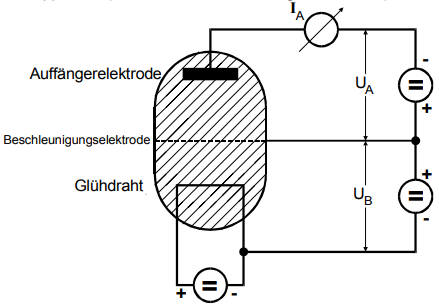
\includegraphics[width=6cm]{aufbau.png}
  \caption{Schematischer Aufbau des Franck-Hertz-Versuchs. \cite[S.116]{kent}}
\end{wrapfigure}
Der Franck-Hertz-Versuch gehört zu den Elektronenstoßexperimenten, mit denen die
diskrete Struktur der Elektronenhüllen untersucht werden kann. In einer abgeschlossenen
 Kammer kommt es dabei zu Wechselwirkungen von Elektronen einer bestimmten Energie und
Hg-Atomen. Diese Wechselwirkungen sind elastische und inelastische Stöße, wobei bei
letzteren die Hg-Atome in den ersten angeregten Zustand versetzt werden. Dabei
nehmen sie die Energie auf, die sich aus der kinetischen Energiedifferenz der Elektronen vor und
nach dem Stoß ergibt:
\begin{align}
\frac{m_\text{0} v_\text{vor}^{2}}{2} - \frac{m_\text{0} v_\text{nach}^{2}}{2} = E_\text{1} - E_\text{0},
\end{align}
mit der Ruhemasse eines Elektrons $m_\text{0}$ und den Geschwindigkeiten $v_\text{vor}$
und $v_\text{nach}$ vor und nach dem Stoß. Die Energie der Elektronen wird mithilfe der
Gegenfeldmethode bestimmt.

\subsection{Versuchsaufbau und Gegenfeldmethode}
In Abbildung 1 ist eine schematische Darstellung der Franck-Hertz-Appartur zu sehen.
Das evakuierte Gefäß beinhaltet einen Tropfen Quecksilber, welches teilweise spontan verdampft
und für einen Gleichgewichtsdampfdruck $p_\text{Sättigung}$ sorgt, welcher nur von der
Umgebungstemperatur abhängig ist.
Der Glühdraht wird mittels Gleichstrom erhitzt, sodass durch den glühelektrischen Effekt
Elektronen austreten. Dem gegenüber steht eine Elektrode, an welcher eine positive
Spannung $U_\text{B}$ anliegt, sodass die Elektronen beschleunigt werden und anschließend
eine kinetische Energie
\begin{align}
\frac{v_\text{vor}^{2}}{2} = e_\text{0} U_\text{B},
\end{align}
wobei $e_\text{0}$ die Elementarladung ist, besitzen, sofern sie vorher die Geschwindigkeit $v = 0$ hatten.
Hinter diese Beschleunigungselektrode wird eine Auffängerelektrode gesetzt. 
Diese ist gegenüber der Beschleunigungselektrode negativ geladen, 
sodass die Elektronen in diesem Teil des Aufbaus abgebremst werden. Nur die Elektronen,
 deren Geschwindigkeit $v_\text{z}$ in Feldrichtung die Ungleichung
\begin{align*}
\frac{m_\text{0}}{2} v_\text{z}^{2} \leq e_\text{0} U_\text{A}
\end{align*}
erfüllt, kommen an der Auffängerelektrode an, die anderen kehren zur Beschleunigungselektrode zurück.

Im Beschleunigungsraum kommt es zwischen den Elektronen und den Hg-Atomen zu
unterschiedlichen Stößen. Ist die Energie der Elektronen gering, treten nur elastische Stöße
auf, bei denen der Energieverlust $\delta E$ des Elektrons nicht von Relevanz ist, da das
Massenverhältnis $\frac{m_\text{0}}{M}$ , welches den Energieverlust bestimmt, sehr klein ist:
\begin{align*}
\delta E = \frac{4 m_\text{0} M}{(m_\text{0} + M)^{2}} \cdot E \approx 1,1 \cdot 10^{-5} E
\end{align*}
wobei $E$ die Energie des Elektrons ist. Während der Energieverlust also zu vernachlässigen ist, 
ist die Richtungsänderung, die das Elektron bei dem Stoß erfährt, trotzdem
relevant. 
Wird die Energie der Elektronen so groß wie die Energiedifferenz
$E_\text{1} - E_\text{0}$ oder größer, kommt es zu inelastischen Stößen zwischen ihnen und den
Hg-Atomen. Auf diese wird der Betrag der Energiedifferenz übertragen, wodurch
sie angeregt werden. Die restliche Energie behält das Elektron. Das Hg-Atom geht vom
ersten angeregten Zustand unter Emission eines Lichtquants mit der Energie 
\begin{align}
h \nu = E_\text{1} - E_\text{0},
\end{align}
wobei $h$ das Plancksche Wirkungsquantum und $\nu$ die Frequenz der emittierten Strahlung
ist, wieder in den Grundzustand zurück.


\begin{wrapfigure}{r}{6.5cm}
  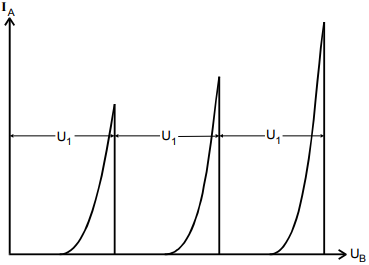
\includegraphics[width=6cm]{peaks.png}
  \caption{Auffängerstrom $I_\text{A}$ in Abhängigkeit der Beschleunigungsspannung $U_\text{B}$. \cite[S.118]{kent}}
\end{wrapfigure}
Bei der Gegenfeldmethode wird nun der Auffängerstrom $I_\text{A}$ in Abhängigkeit 
der Beschleunigungsspannung $U_\text{B}$ betrachtet, während diese kontinuierlich erhöht wird.
Ein schematischer dieses Graphen ist in Abbildung 2 dargestellt. Ist die Beschleunigungsspannung
größer als die Spannung der Auffängerelektrode, wird ein wachsender Strom registriert.
Erreicht die Elektronenenergie den Wert $E_\text{1} - E_\text{0}$, so kommt es zu den genannten
inelastischen Stößen, bei denen die Elektronen ihre Energie verlieren, sodass sie nicht mehr zur
Auffängerelektrode gelangen können. Der Auffängerstrom fällt ab. Ist die Beschleunigungsspannung
groß genug, so kann dieser Prozess mehrfach stattfinden. Die Länge 
\begin{align}
U_\text{1} := \frac{1}{e_\text{0}} (E_\text{1} - E_\text{0}),
\end{align} 
welche die Länge diese periodischen Intervalle bezeichnet, liefert das erste Anregungspotential.

\subsection{Störeinflüsse}
Die tatsächlich beobachtete Kurve des Auffängerstroms weicht aufgrund von einigen Nebeneffekten
ab.

Das Beschleunigungspotential weicht dadurch ab, dass Glühdraht und Beschleunigungselektrode
eine unterschiedliche Austrittsarbeit $\phi_\text{G/B}$ für Elektronen vorweisen, um bei niedriger Temperatur 
bereits höhere Emissionsraten zu erzielen. Es ergibt sich das effektive Beschleunigungspotential
\begin{align}
U_\text{B,eff} = U_\text{B} - \frac{1}{e_\text{0}(\phi_\text{B} - \phi_\text{G})}.
\end{align}
Der Ausdruck $\frac{1}{e_\text{0}}(\phi_\text{B}-\phi_\text{G}$ wird als Kontaktpotential $K$
bezeichnet, um den die resultierende Franck-Hertz-Kurve verschoben ist.

Weiter weisen die Leitungselektronen im Metall des Glühdrahts eine Energieverteilung auf, 
sodass sie mit unterschiedlichen Anfangsgeschwindigkeiten aus diesem austreten und demnach
auch nach der Beschleunigung unterschiedliche Energien besitzen. Die Folge ist, dass die
inelastischen Stöße nicht mehr bei einer bestimmten Beschleunigungsspannung eintreten,
weshalb sich die Kurve flacher den Maxima nähert und stetig bis auf ein Minimum \neq 0 abfällt.
Auch die elastischen Stöße der Elektronen mit den Hg-Atomen zwischen Beschleunigungs- und Auffängerelektrode
sorgen für eine Abflachung und Verbreiterung der Kurve, da die daraus resultierenden Richtungsänderungen
eine Verteilung der relevanten Geschwindigkeitskomponente $v_\text{z}$ hervorrufen. Einige
Elektronen erreichen somit nicht die Auffängerelektrode.

Auch der Dampfdruck $p_\text{Sättigung}$ beeinflusst das Erscheinungsbild der Kurve.
Um eine merkliche Anzahl von Zusammenstößen zwischen Elektronen und Hg-Atomen beobachten zu können,
muss die mittlere freie Weglänge $\overline{w}$ der Atome um den Faktor $1000$ bis $4000$
kleiner als der Abstand $a$ zwischen Beschleunigungs- und Auffängerelektrode sein.
In der kinetischen Gastheorie sind diese in Abhängigkeit der Temperatur $T$ miteinander verknüpft:
\begin{align}
\overline{w} &= \frac{0,0029}{p_\text{Sättigung}},\\
p_\text{Sättigung}(T) &= 5.5 \cdot 10^{7} e^{\frac{-6876}{T}},
\end{align}
wobei $\overline{w}$ in cm, $p_\text{Sättigung}$ in mbar und $T$ in K angegeben werden.
Es gibt also einen Dampfdruckbereich, der sich zur Beobachtung des Effekts besonders gut eignet.
Unterhalb dieses Bereichs sinkt die Wahrscheinlichkeit für die benötigten inelastischen Zusammenstöße,
oberhalb treten zu viele elastische Stöße auf, die mit Richtungsänderung der Elektronenbahnen
einhergehen.